\documentclass[10pt,conference,compsocconf]{IEEEtran}

\usepackage{hyperref}
\usepackage{graphicx}	% For figure environment
\usepackage{bbm}


\begin{document}
\title{CS433-Machine Learning Project 1}

\author{
  Amaury Combes - Vincenzo Bazzucchi - Alexis Montavon\\
}

\maketitle

\begin{abstract}
  The Higgs Boson Kaggle challenge was put in place by physicists in CERN in order to analyze the massive data gathered during their research with the Large Hadron Collider. The idea was to use the best algorithms to predict if a particle collision event was a signal of the Higgs Boson. This challenge was actually one of the biggest ever on Kaggle and we reproduced it in our Machine Learning class at EPFL.
\end{abstract}

\section{Introduction}

The purpose of this first Machine Learning project was for us to find the model that will predict best the signal of a Higgs Boson. In this paper we will present the models and methods we used, the preprocessing we have done, the implementation and give justification for the parameters we chose. We will then explain our results and conclude on what could be improved from here.

\section{Model and Methods}
\label{sec:model}
\subsection{Preprocessing}
After diving into the dataset the first question that came to our attention was how to deal with missing values, represented in the data by $-999.0$. Three options came to mind, setting them to $0$, to the average of every valid values in each feature or to the most frequent value in each feature. We opted for the second option as it seemed more coherent than the first one (although there wasn't any clear differences on the final accuracy result) and cross validation confirmed us that there is no substantial improvement with the third option. This is done by the \textit{mean\_spec} function.\\
We then standardized the dataset to obtain values without a dimension. We implemented a classic standardization function, \textit{standardize}.\\ As we saw in class, linear models are not very rich, so we used the polynomial augmentation technique used in the lab session. This is realized by the \textit{polynomial\_enhancement} function. All the functions used for preprocessing are defined in \textit{preprocessing.py}.\\
Finally, on the advice of different TAs and the article \cite{anderson04}, we chose to train our model on each "categories" based on the jet numbers (this is given by the column \textit{PRI\_jet\_num}). The \textit{category\_iter} generator in \textit{run.py} allows to work on the data one category at a time.

\subsection{Preparing the data for learning}
We performed the preparation of the data matrix before training. This consisted "applying" the degree of the model to the data: given the data matrix $D$, and the degree $d$ we obtained our matrix $X$ by concatenating a column of ones and the successive powers of $D$ : $$X = \left[\vec{1} | D^1 | D^2 | \dots | D^d\right]$$
\textbf{$D^m$ is not the multiplicative power of $D$ }: the element $i,j$ of $D^m$ is $D^m_{i,j}= (D_{i,j})^m$

\subsection{Models}
We implemented and compared different models, all of them are linear models. Therefore one of the parameter we had to tune was the degree of the model.

To compare our models we used k-fold cross validation and computed the \textit{accuracy}. Given the real classification $\vec{y}$ and the predictions we computed $\vec{p}$, both of length $n$ we can simply compute the accuracy $$a(\vec{y}, \vec{p}) = n^{-1}\sum_{i=1}^n \mathbbm{1}\{y_i = p_i\}$$

\subsubsection{Least squares}
Our first attempt consisted in implementing a simple least squares model. As the size of the matrix is relatively small and our machines could inverse it quite easily, we only tried to use the matrix inverse and the pseudo-inverse.

This means that given the data matrix $X$ and the prediction vector $\vec{y}$ we computed the weight vector $\vec{w}$ by
$\vec{w} = X^{-1} \vec{y}$. As the matrix was often singular, we used the pseudo-inverse: $X = U \Sigma V^T$ and then
$$\vec{w} = V \Sigma^{-1} U^T \vec{y}$$
We were surprised by this method as our very first attempt with least squares (with degree 1) gave us an accuracy of $0.744388$ with a 5-fold cross validation and we reached an accuracy of $0.807668$ when training the data enhanced to a degree 8 polynomial.
Least squares is implemented in \textit{least\_squares.py}.\\
After this we tried to train the model on each different category as explained in the preprocessing part. The only remaining thing was to find the best degree for each category and we improved our score to $0.825183780696$.

\subsubsection{Logistic regression} After learning in the lectures about classification, we implemented logistic regression. Given the data matrix, we compute the probability that the point $\vec{x}$ is in category 1 by $\sigma(\vec{x}^T\vec{w})$ where $\sigma(t) = e^t (e^t + 1)^{-1}$. We do so by iteratively minimizing the loss function
$$L(\vec{w}) = \sum^n_{i=1} \ln(1 + \exp{\vec{x}^T \vec{w}}) - y_n \vec{x}^T\vec{w}$$
As the gradient $\nabla L(\vec{w}) = X^T(\sigma(X\vec{w}) - y$ and the Hessian matrix $H_{L}(\vec{w}) = X^TSX$  (where $S_{nn} = \sigma(\vec{x}_n^T w)(1 - \sigma(\vec{x}_n^T\vec{w})$) of the loss function can be easily computed, we found our best results by using Newton's method for minimization which computes $$\vec{w}^{(t+1)} = \vec{w}^{(t)} - \gamma^{(t)} \left(H^{(t)}\right)^{-1}\nabla L\left(\vec{w}^{(t)}\right)$$

Logistic regression is implemented in \textit{logistic.py} and uses minimizers defined in \textit{minimizers.py}.

Using this implementation of logistic regression we improved our accuracy to $0.81632$ using degree $4$ and $\gamma = 0.1$ on the entire matrix. We trained this model on every different category, as we did for least squares, and again obtained a better score of $0.82685350422$.

\subsection{Parameter tuning}
To select the best parameters for our models (the degree of enhancement and the learning rate of the Newton method) we ran several grid searches. In particular, while for the degree a simple grid of integer values was sufficient, for $\gamma$ we first iterated over a logarithmic space ranging from $10^{-5}$ to $1$ and then, once we found a good range, iterated over a linear space from $0.02$ to $1$.\\
During the grid search we did not only try to minimize the loss, but also to maximize the accuracy computed by our cross validation as only minimizing the loss naturally lead to overfitting.

For cross validation we implemented \textit{k-fold cross validation} which, provided the number of folds $k$, splits the data into $k$ chunks: at iteration $i$ the model is trained on chunks $c_{j\neq i}$ and then tested against chunk $c_i$ before incrementing $i$. \\
When working on the entire matrix using high $k$ would result in very slow computations. When working by category, using $k>5$ would result in having chunks too small to have a reliable statistic.

K-fold cross validation is implemented in \textit{cross\_validation.py}.

In the plots we present the accuracies of our models as functions of the degree of the model

\begin{figure}[tbp]
  \centering
  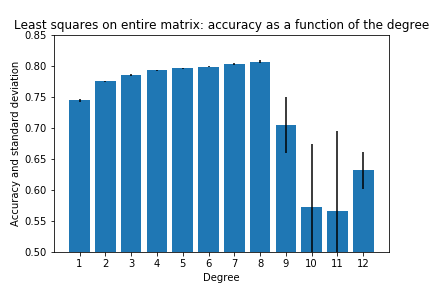
\includegraphics[width=\columnwidth]{ls_deg}
  \caption{Grid search on degrees for Least Squares on entire matrix.}
  \vspace{-3mm}
  \label{fig:denoise-fourier}
\end{figure}
\begin{figure}[tbp]
  \centering
  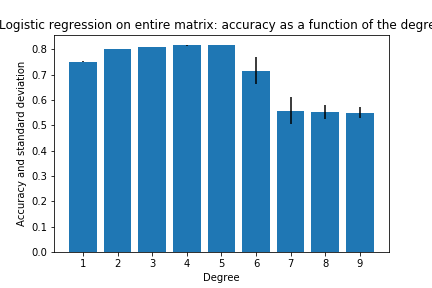
\includegraphics[width=\columnwidth]{lr_deg}
  \caption{Grid search on degrees for Logistic Regression on entire matrix.}
  \vspace{-3mm}
  \label{fig:denoise-fourier}
\end{figure}
\begin{figure}[tbp]
  \centering
  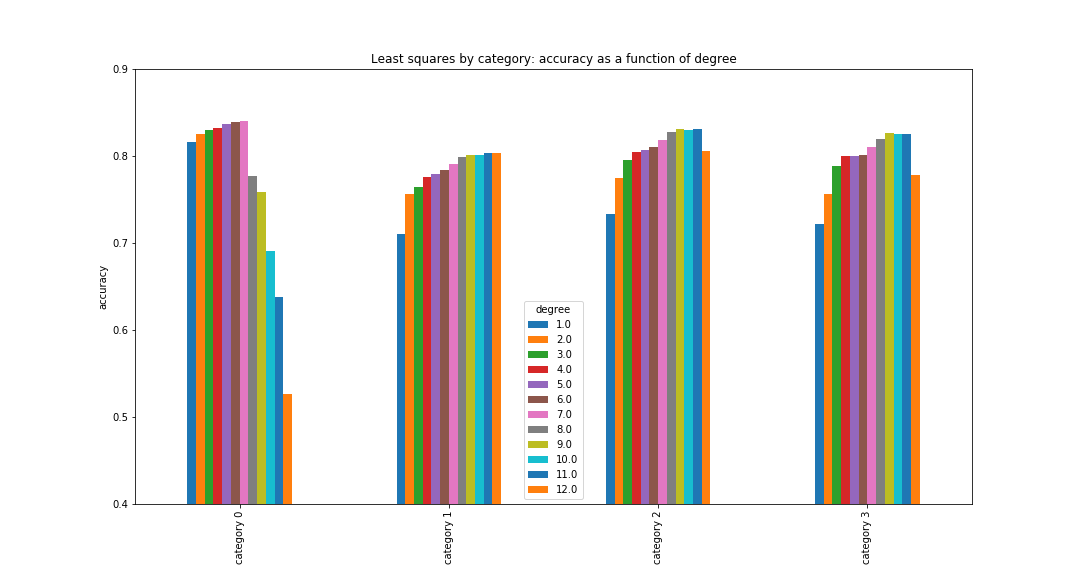
\includegraphics[width=\columnwidth]{ls_cat_deg}
  \caption{Grid search on degrees for Logistic Regression on each category.}
  \vspace{-3mm}
  \label{fig:denoise-fourier}
\end{figure}
\begin{figure}[tbp]
  \centering
  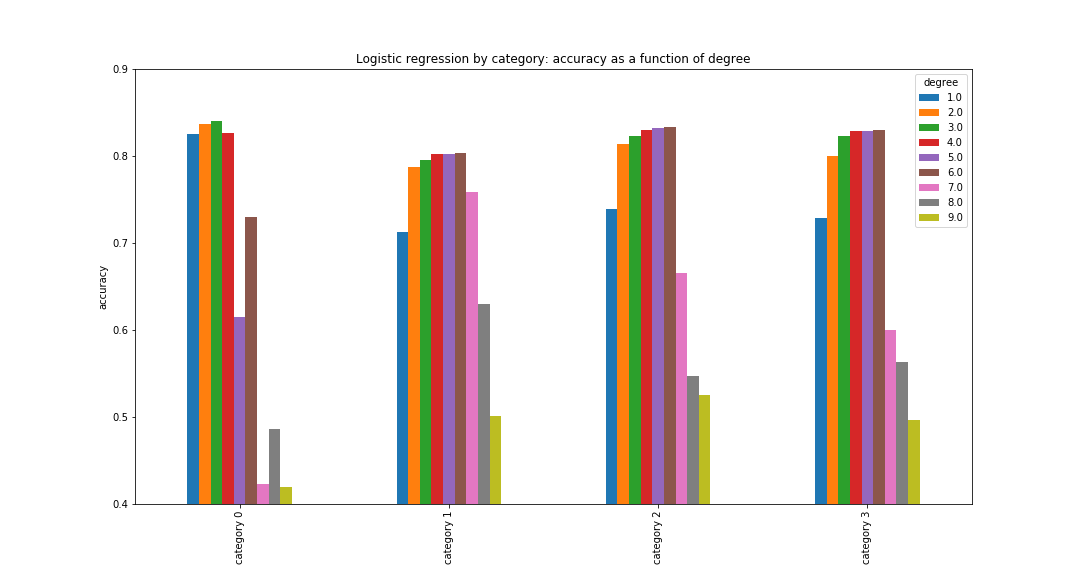
\includegraphics[width=\columnwidth]{lr_cat_deg}
  \caption{Grid search on degrees for Logistic Regression on each category.}
  \vspace{-3mm}
  \label{fig:denoise-fourier}
\end{figure}
\section{Results}

We observe that for the entire matrix the best degrees are 8 for least squares (figure 1) and 5 for logistic regression (figure 2). For the categories we looked for the best parameters for each category and found that the best degrees were
\begin{itemize}
	\item $[7, 11, 11, 9]  $for least squares (figure 3)
	\item $[3, 6, 6, 6] $ for logistic regression (figure 4)
\end{itemize}
For all the logistic regressions we ran $\gamma = 0.1$ caused quick convergence of Newton's method
and acceptable loss.

$\gamma = 0.1$ and the optimal degrees for logistic regression by category gave us our best score on Kaggle: $0.82706$:

\begin{samepage}
\section{Summary}

We tried different linear models under different conditions and parameters and finally concluded that logistic regression produced the best results for this particular challenge. There were some improvements that we considered but we did not have to time to implement them correctly, like model-ensembling or training models separately over clusters of data points located either with a simple PCA or a more  advanced clustering algorithm.
\end{samepage}

\newpage
\bibliographystyle{IEEEtran}
\bibliography{literature}

\end{document}
